\begin{figure}[htbp]
    \centering
    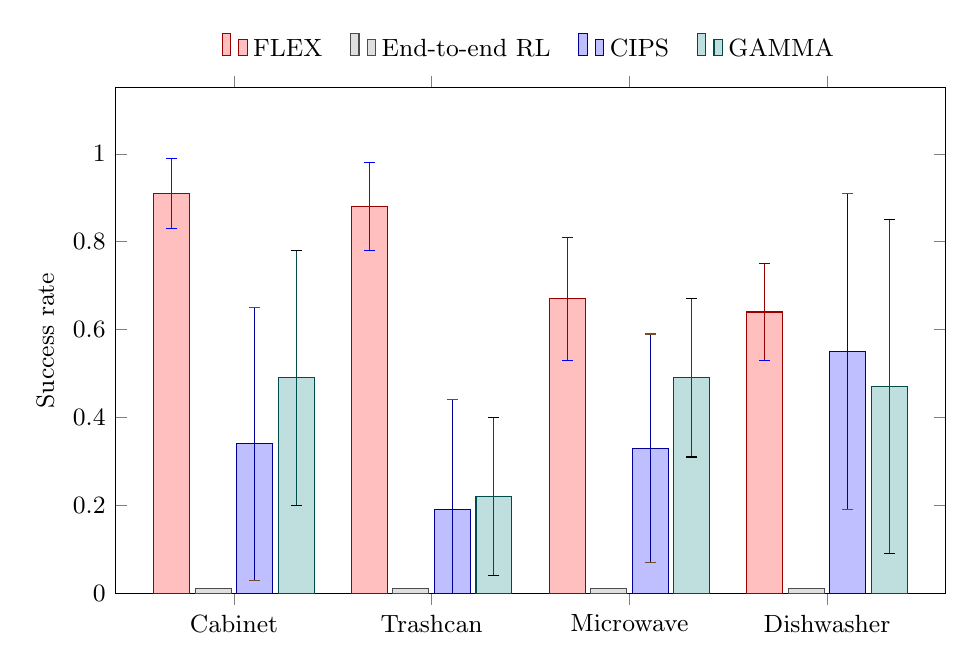
\begin{tikzpicture}
    \begin{axis}[
        ybar=2pt,
        bar width=13pt,
        width=\textwidth, height=8cm,
        enlarge x limits=0.2,
        ymin=0, ymax=1.15,
        ylabel={Success rate},
        symbolic x coords={Cabinet, Trashcan, Microwave, Dishwasher},
        xtick={Cabinet, Trashcan, Microwave, Dishwasher},
        legend style={at={(0.5,1.03)}, anchor=south, legend columns=4,
                      font=\small, draw=none, /tikz/every even column/.append style={column sep=8pt}},
        error bars/y dir=both, error bars/y explicit,
        tick label style={font=\small},
        label style={font=\small},
    ]
    % FLEX
    \addplot+[draw=red!60!black, fill=red!25] coordinates {
        (Cabinet,0.91) +- (0,0.08) (Trashcan,0.88) +- (0,0.10)
        (Microwave,0.67) +- (0,0.14) (Dishwasher,0.64) +- (0,0.11) };
    % End-to-end RL (success rate <= 0.01)
    \addplot+[draw=gray!60!black, fill=gray!25] coordinates {
        (Cabinet,0.01) (Trashcan,0.01) (Microwave,0.01) (Dishwasher,0.01) };
    % CIPS
    \addplot+[draw=blue!60!black, fill=blue!25] coordinates {
        (Cabinet,0.34) +- (0,0.31) (Trashcan,0.19) +- (0,0.25)
        (Microwave,0.33) +- (0,0.26) (Dishwasher,0.55) +- (0,0.36) };
    % GAMMA
    \addplot+[draw=teal!60!black, fill=teal!25] coordinates {
        (Cabinet,0.49) +- (0,0.29) (Trashcan,0.22) +- (0,0.18)
        (Microwave,0.49) +- (0,0.18) (Dishwasher,0.47) +- (0,0.38) };
    \legend{FLEX, End-to-end RL, CIPS, GAMMA}
    \end{axis}
    \end{tikzpicture}
    \caption{Bar-chart visualization of the FLEX success rates reported in \cref{tab:flex_results}, evaluated on novel object instances with the Panda robot. Error bars denote one standard deviation. Cabinets and trashcans are prismatic joints; microwaves and dishwashers are revolute joints. FLEX achieves the highest success rate on every object type while requiring substantially less training than all reinforcement learning baselines (end-to-end RL fails to exceed a $1\%$ success rate within $\geq$10~M time steps).}
    \label{fig:flex_results_bars}
\end{figure}
